This Chapter summarises the structure of the information necessary 
to define a PSHA input model to be used with the OpenQuake-engine.
% -----------------------------------------------------------------------------
% -----------------------------------------------------------------------------
\section{Input Data definition}
\label{sec:hazInputData}
Input data for probabilistic based seismic hazard analysis (Classical, 
Event based, Disaggregation, and UHS) are organised into:
\begin{itemize}
\item A general configuration file;
\item A file describing the Seismic Source System, that is the set of 
    initial source models and associated epistemic uncertainties needed 
    to model the seismic activity in the region of interest.
\item A file describing the Ground Motion System, that is the set of ground 
    motion prediction equations, per tectonic region type, needed to model 
    the ground motion shaking in the region of interest.
\end{itemize}
%
Figure \ref{fig:psha_input} summarises the structure of a PSHA input model
for the OpenQuake-engine and the relationships between the different files.
% ..............................................................................
% . . . . . . . . . . . . . . . . . . . . . . . . . . . . . . . . . . . > Figure
\begin{figure}[!ht]
\centering
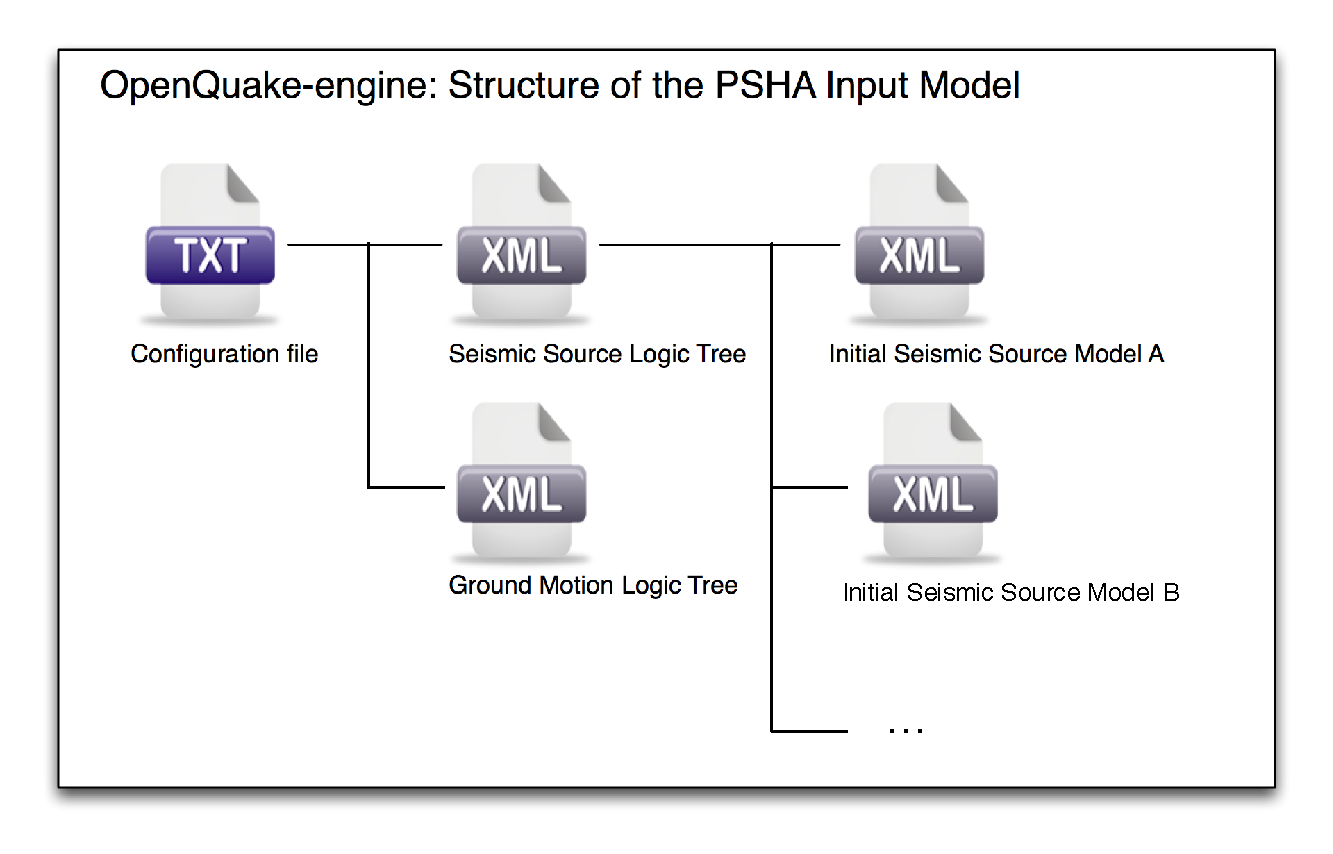
\includegraphics[width=14cm]{./figures/hazard/psha_input_structure.eps}
\caption{PSHA Input Model structure}
\label{fig:psha_input}
\end{figure}
% . . . . . . . . . . . . . . . . . . . . . . . . . . . . . . . . . . . < Figure
% ..............................................................................
% . . . . . . . . . . . . . . . . . . . . . . . . . . . . . . . . . . . . . . .
\subsection{Defining Logic Trees in the OpenQuake engine}
The main components of a logic tree structure in the OpenQuake engine are 
the following:
\begin{description}
    \item[branch]: the simplest component of a logic tree structure. 
    A branch represents a possible interpretation/value assignment of 
    a type of uncertainty. It is fully described by the tuple 
    (parameter/model, weight).
    
    \item[branching set]: a key component in the logic tree structure 
    used by the \gls{acr:oqe}. It groups a set of branches i.e. 
    alternative interpretations of a parameter or a model. Each branching
    set is defined by:
    \begin{itemize}
        \item An ID 
        \item An uncertainty type (for a comprehensive list of the types of 
        uncertainty currently supported see Section )
        \item One or more branches
    \end{itemize}
    
    This set of uncertainties can be applied to the whole initial 
    seismic source input model or just to a subset of seismic source
    data. The sum of the weights/probabilities assigned to the set 
    of branches. 

    \item[branching level]: the largest container. It's not used in 
    modelling uncertainty, but it's useful in maintaining a logic and an 
    order in the structure of the tree.
\end{description}

Below we provide a simple schema illustrating the skeleton of the 
\gls{acr:oqe} logic tree:
\begin{Verbatim}[frame=single, commandchars=\\\{\}, fontsize=\small]
\textcolor{green}{<logicTreeBranchingLevel branchingLevelID=ID>}
    \textcolor{blue}{<logicTreeBranchSet branchSetID=ID}
            \textcolor{blue}{uncertaintyType=TYPE>}
        \textcolor{magenta}{<logicTreeBranch>}
            \textcolor{cyan}{<uncertaintyModel>VALUE</uncertaintyModel>}
            \textcolor{cyan}{<uncertaintyWeight>WEIGHT</uncertaintyWeight>}
        \textcolor{magenta}{</logicTreeBranch>}
    \textcolor{blue}{</logicTreeBranchSet>}
\textcolor{green}{</logicTreeBranchingLevel>}
\end{Verbatim}

A schematic representation of these three objects is provided in Figure 
\ref{glts}. A branching level identifies the position in a tree where
branching occurs while a branch set identifies a collection of branches 
(i.e. individual branches) whose weights sum to 1.\\
%
\begin{figure}[!h]
\centering
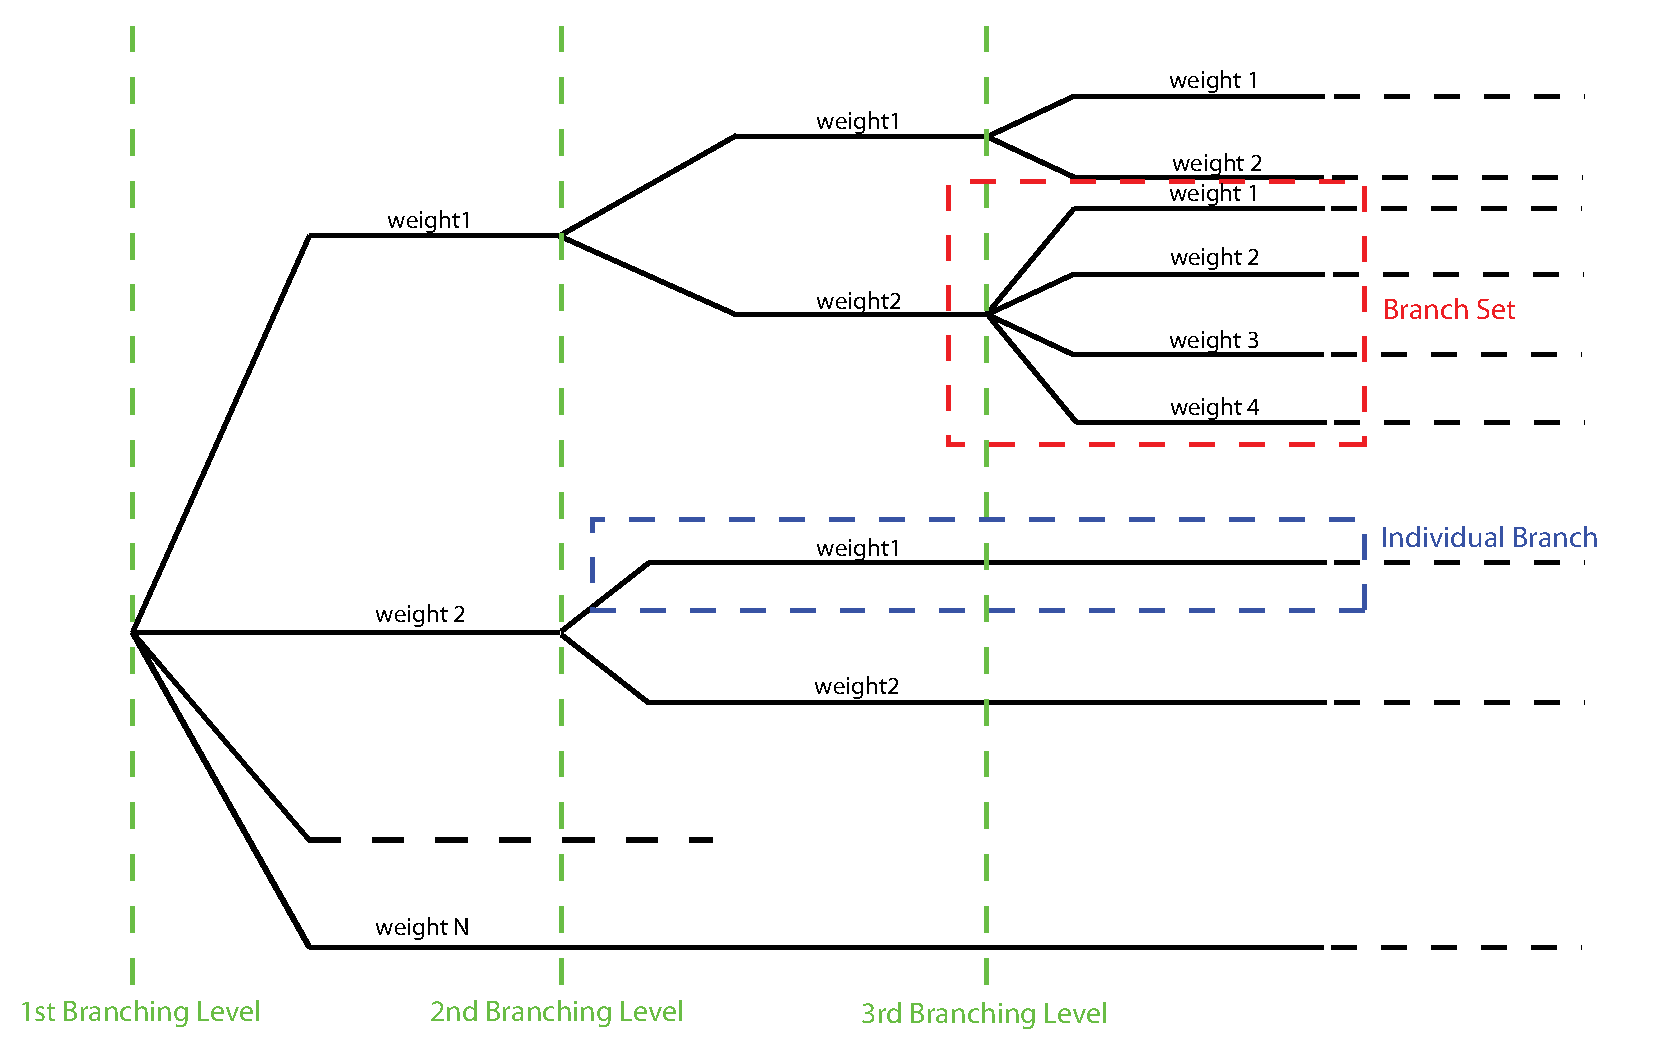
\includegraphics[width=15cm]{./figures/hazard/GenericLogicTreeStructure.eps}
\caption{Generic Logic Tree structure as described in terms of branching 
levels, branch sets, and individual branches.}
\label{glts}
\end{figure}
%
In the NRML schema, a logic tree structure is defined through the 
\Verb+logicTree+ element: 
%
\begin{Verbatim}[frame=single, commandchars=\\\{\}]
<\textcolor{red}{logicTree} logicTreeID="ID">
...
</\textcolor{red}{logicTree}>
\end{Verbatim}
%
A \Verb+logicTree+ contains as a sequence of \Verb+logicTreeBranchingLevel+ 
elements. The position in the sequence specifies in which level of the tree 
the branching level is located. That is, the first 
\texttt{logicTreeBranchingLevel} element in the sequence represents the first 
level in the tree, the second element the second level in the tree, and so on.
%
\begin{Verbatim}[frame=single, commandchars=\\\{\}]
<\textcolor{red}{logicTree} logicTreeID="ID">
	<\textcolor{green}{logicTreeBranchingLevel} branchingLevelID="ID_1">
		...
	</\textcolor{green}{logicTreeBranchingLevel}>
	<\textcolor{green}{logicTreeBranchingLevel} branchingLevelID="ID_2">
		...
	</\textcolor{green}{logicTreeBranchingLevel}>
	....
	<\textcolor{green}{logicTreeBranchingLevel} branchingLevelID="ID_N">
		...
	</\textcolor{green}{logicTreeBranchingLevel}>
</\textcolor{red}{logicTree}>
\end{Verbatim}
No restrictions are present on the number of tree levels that can 
be defined.

A \Verb+logicTreeBranchingLevel+ is defined as a sequence of 
\Verb+logicTreeBranchSet+ elements. Each \Verb+logicTreeBranchSet+ 
defines a particular epistemic uncertainty inside a branching level. 

A branch set has two required attributes (\Verb+branchSetID+ and 
\Verb+uncertaintyType+ (defining the type of epistemic uncertainty 
the branch set is defining))
\begin{Verbatim}[frame=single, commandchars=\\\{\}]
<\textcolor{red}{logicTree} logicTreeID="ID">
...
	<\textcolor{green}{logicTreeBranchingLevel} branchingLevelID="ID_#">
		<\textcolor{blue}{logicTreeBranchSet} branchSetID="ID_1"
			uncertaintyType="UNCERTAINTY_TYPE">
			...
		</\textcolor{blue}{logicTreeBranchSet}>
		<\textcolor{blue}{logicTreeBranchSet} branchSetID="ID_2"
			uncertaintyType="UNCERTAINTY_TYPE">
			...
		</\textcolor{blue}{logicTreeBranchSet}>
		...
		<\textcolor{blue}{logicTreeBranchSet} branchSetID="ID_N"
			uncertaintyType="UNCERTAINTY_TYPE">
			...
		</\textcolor{blue}{logicTreeBranchSet}>
	</\textcolor{green}{logicTreeBranchingLevel}>
...
</\textcolor{red}{logicTree}>
\end{Verbatim}
Possible values for the \Verb+uncertaintyType+ attribute are:
\begin{itemize}
\item \Verb+gmpeModel+: identifying epistemic uncertainties on ground 
motion prediction equations
\item \Verb+sourceModel+: identifying epistemic uncertainties on source models
\item \Verb+maxMagGRRelative+: identifying epistemic uncertainties 
(relative: that is increments) to be added (or subtracted, depending on 
the sign of the increment) to the 
Guten\-berg-Richter maximum magnitude value.
\item \Verb+bGRRelative+: identifying epistemic uncertainties (relative)
to be applied to the Guten\-berg-Richter b value.
\item \Verb+abGRAbsolute+:identifying epistemic uncertainties (absolute: 
that is new values used to replace original values) on the Guten\-berg-Richter
a and b values.
\item \Verb+maxMagGRAbsolute+: identifying epistemic uncertainties 
(absolute) on the Guten\-berg-Richter maximum magnitude.
\end{itemize}
No restrictions are given on the number of branch sets that can be defined 
inside a branching level.

A \Verb+branchSet+ is defined as a sequence of \Verb+logicTreeBranch+ 
elements, each specified by an \Verb+uncertaintyModel+ element (a string 
identifying an uncertainty mod\-el; the content of the string varies with
the uncertaintyType attribute value of the branchSet element) and the
uncertaintyWeight element (specifying the probability/weight associated 
to the uncertaintyModel):
\begin{Verbatim}[frame=single, commandchars=\\\{\}]
<\textcolor{red}{logicTree} logicTreeID="ID">
...
	<\textcolor{green}{logicTreeBranchingLevel} branchingLevelID="ID_#">
		...
		<\textcolor{blue}{logicTreeBranchSet} branchSetID="ID_#"
				uncertaintyType="UNCERTAINTY_TYPE">
			<\textcolor{magenta}{logicTreeBranch} branchID="ID_1">
				<uncertaintyModel>
				UNCERTAINTY_MODEL
				</uncertaintyModel>
				<uncertaintyWeight>
				UNCERTAINTY_WEIGHT
				</uncertaintyWeight>
			</\textcolor{magenta}{logicTreeBranch}>
			...
			<\textcolor{magenta}{logicTreeBranch} branchID="ID_N">
				<uncertaintyModel>
				UNCERTAINTY_MODEL
				</uncertaintyModel>
				<uncertaintyWeight>
				UNCERTAINTY_WEIGHT
				</uncertaintyWeight>
			</\textcolor{magenta}{logicTreeBranch}>
		</\textcolor{blue}{logicTreeBranchSet}>
		...
	</\textcolor{green}{logicTreeBranchingLevel}>
...
</\textcolor{red}{logicTree}>
\end{Verbatim}
Depending on the \Verb+uncertaintyType+ the content of the 
\Verb+<uncertaintyModel>+ element changes:
\begin{itemize}
\item if \Verb+uncertaintyType="gmpeModel"+, the uncertainty model 
contains the name of a ground motion prediction equation (a list of 
available GMPEs are given in appendix A), e.g.:
\begin{Verbatim}[frame=single, commandchars=\\\{\}]
<uncertaintyModel>GMPE_NAME</uncertaintyModel>
\end{Verbatim}
\item if \Verb+uncertaintyType="sourceModel"+, the uncertainty model contains 
the paths to a source model file, e.g.:
\begin{Verbatim}[frame=single, commandchars=\\\{\}]
<uncertaintyModel>SOURCE_MODEL_FILE_PATH</uncertaintyModel>
\end{Verbatim}
\item if \Verb+uncertaintyType="maxMagGRRelative"+, the uncertainty model 
contains the increment to be added (or subtracted, depending on the sign) 
to the Guten\-berg-Richter maximum magnitude:
\begin{Verbatim}[frame=single, commandchars=\\\{\}, samepage=true]
<uncertaintyModel>MAX_MAGNITUDE_INCREMENT</uncertaintyModel>
\end{Verbatim}
\item if \Verb+uncertaintyType="bGRRelative"+, the uncertainty model 
contains the increment to be added (or subtracted, depending on the 
sign) to the Guten\-berg-Richter b value:
\begin{Verbatim}[frame=single, commandchars=\\\{\}, samepage=true]
<uncertaintyModel>B_VALUE_INCREMENT</uncertaintyModel>
\end{Verbatim}
\item if \Verb+uncertaintyType="abGRAbsolute"+, the uncertainty model 
contains one (if the uncertainty apply to a source with only one 
Guten\-berg-Richter magnitude frequency distribution) or more (if the 
source has more than one magnitude frequency distributions) a and b pairs:
\begin{Verbatim}[frame=single, commandchars=\\\{\}, samepage=true]
<uncertaintyModel>
A_VALUE_1 B_VALUE_1
 ... 
A_VALUE_N B_VALUE_N
</uncertaintyModel>
\end{Verbatim}
    \item if \Verb+uncertaintyType="maxMagGRAbsolute"+, the uncertainty 
    model contains one or more (depending on the number of magnitude 
    frequency distributions in the source) Guten\-berg-Richter maximum 
    magnitude values:
%
\begin{Verbatim}[frame=single, commandchars=\\\{\}, samepage=true]
<uncertaintyModel>
MAX_MAGNITUDE_1
 ... 
MAX_MAGNITUDE_N
</uncertaintyModel>
\end{Verbatim}
\end{itemize}
%
No restrictions are given on the number of \Verb+logicTreeBranch+ elements 
that can be defined in a \Verb+logicTreeBranchSet+, as long as the uncertainty 
weights sum to 1.0.

The \Verb+logicTreeBranchSet+ element offers also a number of optional 
attributes allowing for complex tree definitions:
\begin{itemize}
    \item \Verb+applyToBranches+: specifies to which \Verb+logicTreeBranch+ 
    elements (one or more), in the previous branching level, the branch set 
    is linked to. The linking is established by defining the IDs of the 
    branches to link to:
\begin{Verbatim}[frame=single, commandchars=\\\{\}, samepage=true]
applyToBranches="branchID1 branchID2 .... branchIDN"
\end{Verbatim}
    The default is the keyword ALL, which means that a branch set is by default 
    linked to all branches in the previous branching level. By specifying one or 
    more branches to which the branch set links to, non-symmetric logic trees 
    can be defined.
    \item \Verb+applyToSources+: specifies to which source in a source model 
        the uncertainty applies to. Sources are specified in terms of their IDs:
\begin{Verbatim}[frame=single, commandchars=\\\{\}, samepage=true]
applyToSources="srcID1 srcID2 .... srcIDN"
\end{Verbatim}
    \item \Verb+applyToSourceType+: specifies to which source type the 
    uncertainty applies to.  Only one source typology can be defined 
    (\Verb+area+, \Verb+point+, \texttt{simple\-Fault}, 
	\Verb+complexFault+), e.g.:
\begin{Verbatim}[frame=single, commandchars=\\\{\}, samepage=true]
applyToSources="area"
\end{Verbatim}
    \item \Verb+applyToTectonicRegionType+: specifies to which tectonic 
    region type the uncertainty applies to. Only one tectonic region type 
    can be defined (\texttt{Ac\-tive} \texttt{Shallow Crust}, 
    \Verb+Stable Shallow Crust+, \Verb+Subduction Interface+, 
    \texttt{Sub\-duc\-tion} \texttt{IntraSlab}, \texttt{Volcanic}), e.g.:
\begin{Verbatim}[frame=single, commandchars=\\\{\}]
applyToTectonicRegionType="Active Shallow Crust"
\end{Verbatim}
\end{itemize}

% . . . . . . . . . . . . . . . . . . . . . . . . . . . . . . . . . . . . . . .
\subsection{The Seismic Source System}
The Seismic Source System contains the model (or the models) describing 
position, geometry 
and activity of seismic sources of engineering importance for a set of sites
as well as the possible epistemic uncertainties to be incorporated into the 
calculation of seismic hazard.
%
% . . . . . . . . . . . . . . . . . . . . . . . . . . . . . . . . . . . . . . .
\subsubsection{The Seismic Source Logic Tree}
The structure of the Seismic Source Logic Tree consists of at least one 
\gls{branchinglevel}. This branching level is the one used to define the 
\gls{initialseismicsourceinputmodel} (or a number of initial seismic source 
models, see Figure \ref{fig:psha_input}). 

The example provided below shows the simplest Seismic Source Logic Tree 
structure that can be defined in a \gls{pshainputmodel} for \gls{acr:oqe}. 
It's a logic tree with just one branching level containing 
one \gls{branchset} with one branch used to define the initial seismic source 
model (its weight will be equal to one).
\begin{Verbatim}[frame=single, commandchars=\\\{\}, fontsize=\small,
    firstnumber=1, numbers=left, numbersep=2pt]
<?xml version="1.0" encoding="UTF-8"?>
<nrml xmlns:gml="http://www.opengis.net/gml"
      xmlns="http://openquake.org/xmlns/nrml/0.4">
    <logicTree logicTreeID="lt1">
        <logicTreeBranchingLevel branchingLevelID="bl1">
            <logicTreeBranchSet uncertaintyType="sourceModel"
                                branchSetID="bs1">
                <logicTreeBranch branchID="b1">
                    <uncertaintyModel>seismic_source_model.xml
                    </uncertaintyModel>
                    <uncertaintyWeight>1.0</uncertaintyWeight>
                </logicTreeBranch>
            </logicTreeBranchSet>
        </logicTreeBranchingLevel>
    </logicTree>
</nrml>
\end{Verbatim}

The optional branching levels will contain rules that modify parameters 
of the sources in the initial seismic source model.

For example, if the epistemic uncertainties to be considered are
source geometry and maximum magnitude, the modeller can create a logic tree
structure with three initial seismic source models (each one exploring a 
different definition of the geometry of sources) and one branching level 
accounting for the epistemic uncertainty on the maximum magnitude.
 
Below we provide an example of such logic tree structure.
\begin{Verbatim}[frame=single, commandchars=\\\{\}, fontsize=\small,
    firstnumber=1, numbers=left, numbersep=2pt]
<?xml version="1.0" encoding="UTF-8"?>
<nrml xmlns:gml="http://www.opengis.net/gml"
      xmlns="http://openquake.org/xmlns/nrml/0.4">
    <logicTree logicTreeID="lt1">

        <logicTreeBranchingLevel branchingLevelID="bl1">
            <logicTreeBranchSet uncertaintyType="sourceModel"
                                branchSetID="bs1">
                <logicTreeBranch branchID="b1">
                    <uncertaintyModel>seismic_source_model_A.xml
                    </uncertaintyModel>
                    <uncertaintyWeight>0.2</uncertaintyWeight>
                </logicTreeBranch>
                <logicTreeBranch branchID="b2">
                    <uncertaintyModel>seismic_source_model_B.xml
                    </uncertaintyModel>
                    <uncertaintyWeight>0.3</uncertaintyWeight>
                </logicTreeBranch>
                <logicTreeBranch branchID="b3">
                    <uncertaintyModel>seismic_source_model_C.xml
                    </uncertaintyModel>
                    <uncertaintyWeight>0.5</uncertaintyWeight>
                </logicTreeBranch>
            </logicTreeBranchSet>
        </logicTreeBranchingLevel>

        <logicTreeBranchingLevel branchingLevelID="bl2">
            <logicTreeBranchSet branchSetID="bs21" 
                    uncertaintyType="maxMagGRRelative">
                <logicTreeBranch branchID="b211">
                    <uncertaintyModel>+0.0</uncertaintyModel>
                    <uncertaintyWeight>0.6</uncertaintyWeight>
                </logicTreeBranch>
                <logicTreeBranch branchID="b212">
                    <uncertaintyModel>+0.5</uncertaintyModel>
                    <uncertaintyWeight>0.4</uncertaintyWeight>
                </logicTreeBranch>
            </logicTreeBranchSet>
        </logicTreeBranchingLevel>

    </logicTree>
</nrml>
\end{Verbatim}
Note that the uncertainty on the maximum magnitude is specified in terms 
of relative increments with respect to the initial maximum magnitude 
defined for each source in the initial seismic source models.
%
% . . . . . . . . . . . . . . . . . . . . . . . . . . . . . . . . . . . . . . .
\subsubsection{The Seismic Source Model}
\index{Input!Configuration file} 
The structure of the xml file representing the seismic source 
model corresponds to a list of sources, each one modelled using 
one out of the five typologies currently supported.
Below we provide a schematic example of a seismic source model.
\begin{Verbatim}[frame=single, commandchars=\\\{\}, fontsize=\small]
<\textcolor{red}{sourceModel} gml:id="ID">
	...
	<\textcolor{green}{areaSource} gml:id="SOURCE_ID">
		<gml:name>SOURCE_NAME</gml:name>
		<tectonicRegion>TECT_REGION_TYPE</tectonicRegion>
		...
	</\textcolor{green}{areaSource}>
	...
	<\textcolor{green}{pointSource} gml:id="SOURCE_ID">
		<gml:name>SOURCE_NAME</gml:name>
		<tectonicRegion>TECT_REGION_TYPE</tectonicRegion>
		...
	</\textcolor{green}{pointSource}>
	...
	<\textcolor{green}{simpleFaultSource} gml:id="SOURCE_ID">
		<gml:name>SOURCE_NAME</gml:name>
		<tectonicRegion>TECT_REGION_TYPE</tectonicRegion>
		...
	</\textcolor{green}{simpleFaultSource}>
	...
	<\textcolor{green}{complexFaultSource} gml:id="SOURCE_ID">
		<gml:name>SOURCE_NAME</gml:name>
		<tectonicRegion>TECT_REGION_TYPE</tectonicRegion>
		...
	</\textcolor{green}{complexFaultSource}>
	...
</\textcolor{red}{sourceModel}>
\end{Verbatim}

%
% . . . . . . . . . . . . . . . . . . . . . . . . . . . . . . . . . . . . . . .
\subsection{The Ground Motion System}
\index{Input!Ground motion system} 
The Ground Motion System defines the models and the possible epistemic 
uncertainties related to ground motion modelling to be incorporated 
into the calculation.
%
% . . . . . . . . . . . . . . . . . . . . . . . . . . . . . . . . . . . . . . .
\subsubsection{The Ground Motion Logic Tree}
\index{Input!Ground motion logic tree} 
\label{ref:gmlt_example}
The structure of the \gls{groundmotionlogictree} consists of a list 
of ground motion prediction equations for each tectonic region used to
characterise the sources in the PSHA input model.

The example below shows a simple \gls{groundmotionlogictree}. 
This logic tree assumes that all the sources in the PSHA input model 
belong to ``Active Shallow Crust'' and uses for calculation the 
\citet{chiou2008} \gls{acr:gmpe}.
\begin{Verbatim}[frame=single, commandchars=\\\{\}, fontsize=\small,
    firstnumber=1, numbers=left, numbersep=2pt]
<?xml version="1.0" encoding="UTF-8"?>
<nrml xmlns:gml="http://www.opengis.net/gml"
      xmlns="http://openquake.org/xmlns/nrml/0.4">
    <logicTree logicTreeID='lt1'>
        <logicTreeBranchingLevel branchingLevelID="bl1">
            <logicTreeBranchSet uncertaintyType="gmpeModel" 
                    branchSetID="bs1"
                    applyToTectonicRegionType="Active Shallow Crust">

                <logicTreeBranch branchID="b1">
                    <uncertaintyModel>
                    ChiouYoungs2008
                    </uncertaintyModel>
                    <uncertaintyWeight>1.0</uncertaintyWeight>
                </logicTreeBranch>

            </logicTreeBranchSet>
        </logicTreeBranchingLevel>
    </logicTree>
</nrml>
\end{Verbatim}
%
% . . . . . . . . . . . . . . . . . . . . . . . . . . . . . . . . . . . . . . . 
% . . . . . . . . . . . . . . . . . . . . . . . . . . . . . . . . . . . . . . . 
\subsection{Configuration file}
\index{Input!Configuration file} 
\label{sec:conf_file}
The configuration file is the primary file controlling both the 
definition of the input model as well as parameters governing the 
calculation. We illustrate in the following different examples of 
the configuration file addressing different typologies of seismic 
hazard calculation.
\subsubsection[Calculation of a hazard map and hazard curves using 
    classical PSHA]{Calculation of a hazard map and hazard curves using 
    the classical PSHA methodology}
\label{sec:config_classical_PSHA}
%
In the following we describe the overall structure and the
most typical parameters of a configuration file to be used for the 
computation of a seismic hazard map using a classical PSHA methodology.
\begin{itemize}
\item \textbf{Calculation type and model info}
\begin{Verbatim}[frame=single, commandchars=\\\{\}, fontsize=\small,
    numbers=left, numbersep=2pt]
[general]
description = A demo OpenQuake-engine .ini file for classical PSHA
calculation_mode = classical
random_seed = 1024
\end{Verbatim}

In this section the user specifies the following parameters:
\begin{itemize}
    \item \texttt{description}: a parameter that can be used to designate 
        the model 
    \item \texttt{calculation\_mode}: it is used to set the kind 
        of calculation. In this case it corresponds to \texttt{classical}.
        We'll describe alternative options later on.
    \item \texttt{random\_seed}: is used to control the random generator 
        so that when montecarlo procedures are used calculations are 
        replicable (if the same \texttt{random\_seed} is used).
\end{itemize}
%
\item \textbf{Geometry of the area (or the sites) where hazard is computed}
    \hfill \\
This section is used to specify where hazard will be computed. Two 
option are available. 

The first one consists on defining a polygon 
(usually a rectangle) and a distance (in km) used to discretize the 
polygon area. The polygon is defined by a list of longitude-latitude tuples.

An example is provided below.
\begin{Verbatim}[frame=single, commandchars=\\\{\}, fontsize=\small,
    firstnumber=5, numbers=left, numbersep=2pt]
[geometry]
region = 10.0 43.0, 12.0 43.0, 12.0 46.0, 10.0 46.0
\# km
region_grid_spacing = 10.0
\end{Verbatim}

The second option allows the definition of a number of sites where 
the hazard will be computed. An example is provided below.
\begin{Verbatim}[frame=single, commandchars=\\\{\}, fontsize=\small,
    firstnumber=5, numbers=left, numbersep=2pt]
[geometry]
sites = 10.0 43.0, 12.0 43.0, 12.0 46.0, 10.0 46.0
\end{Verbatim}

If the list of sites is too long the user can specify the name 
of a .csv file as it is snown below
\begin{Verbatim}[frame=single, commandchars=\\\{\}, fontsize=\small,
    firstnumber=5, numbers=left, numbersep=2pt]
[geometry]
sites\_csv = <name_of_the_csv_file>
\end{Verbatim}
%
\item \textbf{Logic tree sampling} \hfill \\
    The \gls{acr:oqe} provides two options for processing the whole 
    logic tree structure. The first option uses Montecarlo sampling;
    the user in this case specifies a number of realisations. 

    In the second option all the possible realisations are created. 
    Below we provide an example for the latter option.
    In this example we set the \texttt{number\-\_of\-\_logic\_tree\_samples}
    to 0. \gls{acr:oqe} will perform a complete enumeration of all 
    the possible paths from the roots to the leaves of the logic tree 
    structure.
\begin{Verbatim}[frame=single, commandchars=\\\{\}, fontsize=\small,
    firstnumber=9, numbers=left, numbersep=2pt]
[logic_tree]
number_of_logic_tree_samples = 0
\end{Verbatim}
    If the seismic source logic tree and the ground motion
    logic tree do not contain epistemic uncertainties the engine will
    create a single PSHA input.
%
\item \textbf{Parameters controlling the construction of the earthquake 
    rupture forecast}
\begin{Verbatim}[frame=single, commandchars=\\\{\}, fontsize=\small,
    firstnumber=11, numbers=left, numbersep=2pt]
[erf]
# km
rupture_mesh_spacing = 5
width_of_mfd_bin = 0.1
# km
area_source_discretization = 10
\end{Verbatim}
This section of the configuration file is used to specify the 
level of discretization of the mesh representing faults, of the grid
used to delineate the area sources and, of the magnitude-frequency 
distribution. 
Note that the lower is the mesh spacing (or the bin width) the higher 
are the precision in the representation and the computation demand.
%
\item \textbf{Parameters describing site conditions}
\begin{Verbatim}[frame=single, commandchars=\\\{\}, fontsize=\small,
    firstnumber=17, numbers=left, numbersep=2pt]
[site_params]
reference_vs30_type = measured
reference_vs30_value = 760.0
reference_depth_to_2pt5km_per_sec = 5.0
reference_depth_to_1pt0km_per_sec = 100.0
\end{Verbatim}
In this section the user specifies local soil conditions. The simplest
solution is to define uniform site conditions (i.e. all the sites have 
the same soil conditions). Alternatively it's possible to define 
spatially variable soil properties in a separate file; the engine will
then assign to each investigation site the appropriate characteristics.
%
\begin{Verbatim}[frame=single, commandchars=\\\{\}, fontsize=\small,
    firstnumber=17, numbers=left, numbersep=2pt]
[site_params]
site_model_file = ../_site_model/site_model.xml
\end{Verbatim}

The file containing the site model has the following 
structure:
\begin{Verbatim}[frame=single, commandchars=\\\{\}, fontsize=\small]
<?xml version="1.0" encoding="utf-8"?>
<nrml xmlns:gml="http://www.opengis.net/gml"
      xmlns="http://openquake.org/xmlns/nrml/0.4">
    <siteModel>
        <site lon="10.0" lat="40.0" vs30="800.0" 
            vs30Type="inferred" 
            z1pt0="19.367196734" z2pt5="0.588625072259" />
        <site lon="10.1" lat="40.0" vs30="800.0" 
            vs30Type="inferred" 
            z1pt0="19.367196734" z2pt5="0.588625072259" />
        <site lon="10.2" lat="40.0" vs30="800.0" 
            vs30Type="inferred" 
            z1pt0="19.367196734" z2pt5="0.588625072259" />
        <site lon="10.3" lat="40.0" vs30="800.0" 
            vs30Type="inferred" 
            z1pt0="19.367196734" z2pt5="0.588625072259" />
        <site lon="10.4" lat="40.0" vs30="800.0" 
            vs30Type="inferred" 
            z1pt0="19.367196734" z2pt5="0.588625072259" />
        ...
    </siteModel>
</nrml>
\end{Verbatim}

%
\item \textbf{Calculation configuration}
\phantomsection
\label{sec:calculation_configuration}
\begin{Verbatim}[frame=single, commandchars=\\\{\}, fontsize=\small,
     firstnumber=22, numbers=left, numbersep=2pt]
[calculation]
source_model_logic_tree_file = source_model_logic_tree.xml
gsim_logic_tree_file = gmpe_logic_tree.xml
# years
investigation_time = 50.0
intensity_measure_types_and_levels = \{"PGA": [0.005, ..., 2.13]\} 
truncation_level = 3
# km
maximum_distance = 200.0
\end{Verbatim}
This section of the \gls{acr:oqe} configuration file specifies the 
parameters that
are relevant for the calculation of hazard. These include the names of
the two files containing the Seismic Source System and the Ground 
Motion System, the duration of the time window used to compute the 
hazard, the ground motion intensity measure types and levels for 
which the probability of exceedence will be computed, the level of
truncation of the gaussian 
distribution of the logarithm of ground motion used in the calculation 
of hazard and the maximum integration distance (i.e. the distance within 
which sources will contribute to the computation of the hazard).
%
\item \textbf{Output}
\begin{Verbatim}[frame=single, commandchars=\\\{\}, fontsize=\small,
    firstnumber=32, numbers=left, numbersep=2pt]
[output]
export_dir = out/
# given the specified `intensity_measure_types_and_levels`
quantile_hazard_curves =
poes_hazard_maps = 0.1
\end{Verbatim}
The final section of the configuration file is the one that contains 
the parameters controlling the typology of output to be produced.
%
\end{itemize}
%
%\input{config_file_event_based.tex}
%

\subsubsection{Seismic hazard disaggregation}
%
In this section we describe the structure of the configutation 
file to be used to complete a seismic hazard disaggregation. 
Since only a few parts of the standard configuration file need to 
be changed we'll use the description given in Section 
\ref{sec:config_classical_PSHA} at page 
\pageref{sec:config_classical_PSHA} as a reference and we'll 
emphasize in the following major differences.
%
\begin{itemize}
%
\item \textbf{Calculation type and model info}
\begin{Verbatim}[frame=single, commandchars=\\\{\}, fontsize=\small]
[general]
description = A demo .ini file for PSHA disaggregation
calculation_mode = disaggregation
random_seed = 1024
\end{Verbatim}
The calculation mode parameter in this case is set as 
\texttt{disaggregation}.
%
\item \textbf{Geometry of the area (or the sites) where hazard is computed}
\begin{Verbatim}[frame=single, commandchars=\\\{\}, fontsize=\small]
[geometry]
sites = 11.0 44.5


\end{Verbatim}
In the section it will be necessary to specify the geographic 
coordinates of the site (or the sites) where the disaggregation
will be performed.
%
\item \textbf{Disaggregation parameters}
\begin{Verbatim}[frame=single, commandchars=\\\{\}, fontsize=\small]
[disaggregation]
poes_disagg = 0.02, 0.1
mag_bin_width = 1.0
distance_bin_width = 25.0
# decimal degrees
coordinate_bin_width = 1.5
num_epsilon_bins = 3
\end{Verbatim}
With the disaggregation settings shown above we'll disaggregate the intensity
measure levels with 10\% and 2\% probability of exceedance using the
\texttt{in\-ves\-ti\-gation\_time} and the intensity measure types 
defined in the ``Calculation configuration'' section of the OpenQuake
configuration file (see page \pageref{sec:calculation_configuration}). 
\end{itemize}

\subsubsection{Event based PSHA}
%
In the following we describe the sections of the configuration file 
that are required to complete event based PSHA calculations 
\begin{enumerate}
\item \textbf{Calculation type and model info} \hfill \\
    This part is almost identical to the corresponding one 
    described in section \ref{sec:config_classical_PSHA}. Note
    the setting of the \texttt{cal\-cu\-lation\_mode} parameter
    which now corresponds to \texttt{event\_based}.
\begin{Verbatim}[frame=single, commandchars=\\\{\}, fontsize=\small,
    numbers=left, numbersep=2pt]
[general]
description = A demo OpenQuake-engine .ini file for classical PSHA
calculation_mode = event_based
random_seed = 1024
\end{Verbatim}
%
\item \textbf{Event based} \hfill \\
This is section is used to specify the number of stochastic 
event sets to be generated for each logic tree realisation 
(each stochastic event set represents a potential realisation of seismicity
during the \texttt{in\-ves\-ti\-gation\_time} specified in the 
\texttt{calculation\_configuration} part).
Additionally, in this section the user can specify the spatial correlation
model to be used in case for the generation of ground motion fields. 
\begin{Verbatim}[frame=single, commandchars=\\\{\}, fontsize=\small]
[event_based_params]
ses_per_logic_tree_path = 5
ground_motion_correlation_model = JB2009
ground_motion_correlation_params = {"vs30_clustering": true}
\end{Verbatim}
%
\item \textbf{Output} \hfill \\
This part substitutes the \texttt{Output} part described in 
the configuration file example described in the section 
\ref{sec:config_classical_PSHA}
at page \pageref{sec:config_classical_PSHA}.
\begin{Verbatim}[frame=single, commandchars=\\\{\}, fontsize=\small]
[output]
export_dir = /tmp/xxx
complete_logic_tree_ses = true
complete_logic_tree_gmf = true
ground_motion_fields = true
# post-process ground motion fields into hazard curves,
# given the specified `intensity_measure_types_and_levels`
hazard_curves_from_gmfs = true
mean_hazard_curves = true
quantile_hazard_curves = 0.15, 0.5, 0.85
poes_hazard_maps = 0.1, 0.2
\end{Verbatim}
%
\end{enumerate}

